\section{Implied liquidity as a constrained network}
\label{sec:implied}

An implied-IN opportunity combines outright orders to offer a spread; an implied-OUT opportunity combines a spread with other legs to offer an outright. CME documents both constructions. It also specifies that implied bids do not trade directly against implied offers, that implication is unavailable in nonmatching phases, and that some executable implied quantities are not disseminated \citep{CMEImplied}. Consequently, neither an unrestricted network optimizer nor a sum of displayed quantities is a faithful description of the mechanism.

\subsection{Signed legs and quote conventions}

Let $e_j$ be the unit vector for underlying future $j$. A strategy is described by an integer leg vector $\ell\in\Z^d$. Buying a one-for-one calendar $A-B$ creates
\begin{equation}
 \ell_{AB}=e_A-e_B.
\end{equation}
With common multiplier $m$, its difference quote is $p_A-p_B$ and its signed underlying quote value is $m(p_A-p_B)$. With unequal multipliers, currencies, or ratio conventions, the conversion must instead be performed leg by leg. A raw subtraction of two displayed numbers need not be financially meaningful.

For strategy executions $x_k\in\N$,
\begin{equation}
 \Delta z=\sum_kx_k\ell_k=Lx,
 \qquad L=[\ell_1\ \cdots\ \ell_K].
\label{eq:legs}
\end{equation}
The matrix $L$ records signed positions. It is distinct from the nonnegative matrix that records consumption of available orders.

\subsection{Recipes consume shared inputs}

Enumerate a \emph{declared} set of feasible matching recipes $k=1,\ldots,K$. A recipe includes its aggressor form, required resting orders, prices, leg ratios, and phase eligibility. Let $A_{ik}$ be the number of contracts consumed from resting order $i$ per unit of recipe $k$. With available capacities $q_i$, any execution vector must satisfy
\begin{equation}
 x\in\Z_+^K,\qquad Ax\le q.
\label{eq:resources}
\end{equation}
This is a necessary resource condition. It is sufficient only for the explicitly declared simultaneous-allocation model with no further compatibility or sequencing restrictions. The exchange chooses according to its priority rules; it is not asserted to solve a global maximum-volume integer program.

\begin{example}[Eleven indicated contracts, eight jointly feasible]\label{ex:shared}
Consider three CL maturities and ordinary resting orders: an $A$ ask for eight contracts at 75.01, a $B$ bid for five at 74.81, and a $C$ bid for six at 74.51. All prices are dollars per barrel. There is an implied ask for five $A-B$ spreads at 0.20 and an implied ask for six $A-C$ spreads at 0.50. In the restricted recipe model,
\begin{equation}
 A=\begin{pmatrix}1&1\\1&0\\0&1\end{pmatrix},\quad
 q=\begin{pmatrix}8\\5\\6\end{pmatrix},\quad
 x_1\le5,\quad x_2\le6,\quad x_1+x_2\le8.
\end{equation}
Five plus six is eleven, but both constructions use the same $A$ ask. At most eight spread contracts can execute jointly. The allocation $(x_1,x_2)=(5,3)$ consumes $(8,5,3)$ underlying contracts and creates aggressor positions $(8,-5,-3)$.
\end{example}

The signed entry quote value for that allocation is
\begin{equation}
 1000[8(75.01)-5(74.81)-3(74.51)]
 =1000[5(0.20)+3(0.50)]=\$2{,}500.
\end{equation}
This is a difference valuation for the leg ledger, not an upfront premium. Its subsequent variation depends on the settlement changes of all three maturities.

An implied-OUT calculation in a separate matching opportunity is equally direct: an $A-B$ ask at 0.20 for four contracts and a $B$ ask at 74.82 for seven imply an $A$ ask at 75.02 for at most four. The signs are essential: buying the spread gives $+A-B$, and buying $B$ cancels the $-B$ leg. Two sell orders in unrelated maturities would not produce this exposure.

\begin{figure}[htbp]
\centering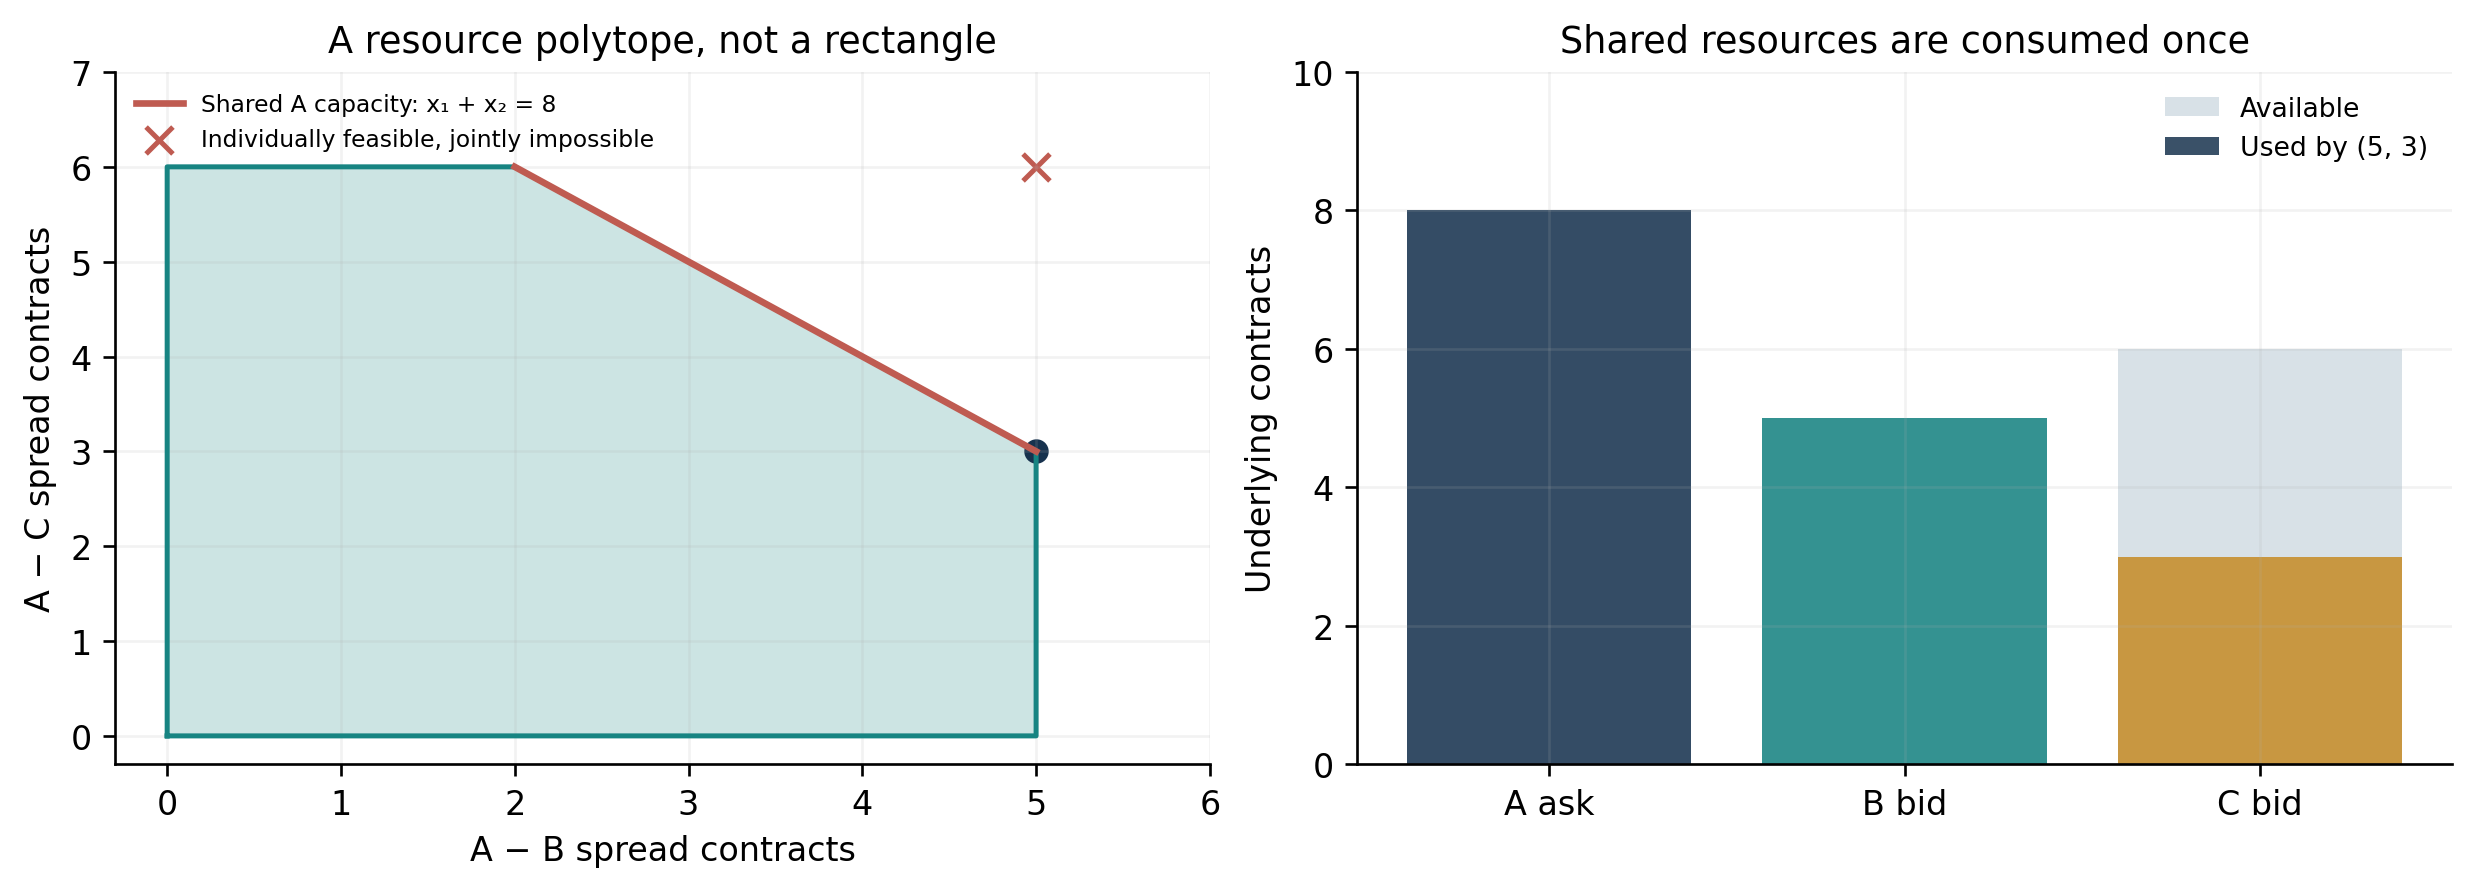
\includegraphics[width=\textwidth]{figures/03_implied.png}
\caption{Shared-resource geometry in Example~\ref{ex:shared}. The feasible polygon removes the upper-right corner of the rectangle suggested by individual implied quantities. The point $(5,6)$ is infeasible; $(5,3)$ uses the common $A$ capacity exactly.}
\label{fig:implied}
\end{figure}

\subsection{A dual certificate for available liquidity}

For nonnegative recipe weights $w_k$, consider the continuous relaxation
\begin{equation}
 \max\{w^\top x:Ax\le q,\ x\ge0\}.
\label{eq:primal}
\end{equation}
Weights may measure spread lots in a common unit or another declared objective. Counting unrelated multi-leg strategies as if one unit meant the same exposure is not generally useful.

\begin{proposition}[Resource-price certificate]\label{prop:dual}
For any $\lambda\ge0$ satisfying $A^\top\lambda\ge w$, every feasible integer or real allocation satisfies
\begin{equation}
 w^\top x\le\lambda^\top q.
\end{equation}
If a feasible $x^*$ and such a $\lambda^*$ attain equality, both certify the optimum of the relaxation, and $x^*$ is also integer-optimal if integer valued.
\end{proposition}
\begin{proof}
Nonnegativity gives $w^\top x\le\lambda^\top Ax\le\lambda^\top q$. Equality at a feasible pair leaves no room for improvement.
\end{proof}

In Example~\ref{ex:shared}, $w=(1,1)$ and $\lambda=(1,0,0)$ give the upper bound eight. The feasible integer point $(5,3)$ attains it. The entire bottleneck is certified by the shared $A$ order. In more general ratio systems, the relaxation need not be integral; its value remains an upper bound and must not be reported as an executable contract count without an integer solution.

\subsection{Price potentials and cycles}

For maturities with a common price convention, assign a scalar potential $p_j$ to each vertex and difference quote $c_{ij}=p_i-p_j$ to a calendar edge. For any closed cycle,
\begin{equation}
 c_{12}+c_{23}+\cdots+c_{k1}=0.
\label{eq:cycle}
\end{equation}
Conversely, on a connected graph, antisymmetric edge values with zero sum around every cycle admit vertex potentials, unique up to an additive constant. To construct them, fix one vertex value and sum edge differences along a path; zero cycle sums make the result path independent.

This identity describes consistent difference valuations. For actual bid and ask executions, the corresponding no-arbitrage statement requires a \emph{jointly feasible} zero-net-leg trade cycle, correct multipliers, fees, and settlement conventions. If its signed entry value is negative and its net position is zero, the settlement identity in Section~\ref{sec:settlement} converts the negative entry value into a positive gain before costs. A displayed cycle with insufficient shared capacity or disallowed implied-to-implied matching provides no such executable transaction.

The topology therefore has two layers: signed exposure describes what a strategy creates, and nonnegative capacity describes which strategies can coexist. A useful model preserves both.
\FloatBarrier
